\section{Monotone functions}
A function $f: L \to L$ is monotone when $\forall x,y \in S : x \sqsubseteq y \Rightarrow f(x) \sqsubseteq f(y)$.
Being monotone does not imply that the function is increasing.
All constant functions are monotone.

If we look at the least upper bound and greatest lower bound functions they are monotone in both arguments.
This means that we can apply the least upper bound function on two arguments and be certain that it will never decrease.
This is an important reqiurement for the fixed-point theorem which will be presented in the next section.

\section{Fixed-point}
For the static analysis of a program we need a theorem that can find the best approximation of some dataflow problem.
Because we will generally consider problems that are undecidable \todo{ref til intro om undecidable problems} we need a framework that overestimate the answer, and thus makes an approximation.

This framework will be based on the fixed-points theorem which states the following (quoted from \citet[p.~13]{schwartzbach}):

\begin{definition}{Fixed-point theorem}
In a lattice L with finite height, every monotone function $f$ has a unique least fixed-point defined as
\[ fix(f) = \bigsqcup_{i \ge 0} f^i(\bot) \]

for which $f(fix(f)) = fix(f)$
\end{definition}

\noindent
The proof of this theorem can be found in \citep[p.~13]{schwartzbach}.

This theorem enables us to find an approximation to an undecidable problem by walking up the lattice until a fixed-point is reached.
This computation has been illustrated in \cref{lattice_walk} where the analysis starts at $\bot$ and end in the fixed-point which is the approximation to the problem at hand.

\begin{figure}
\begin{center}
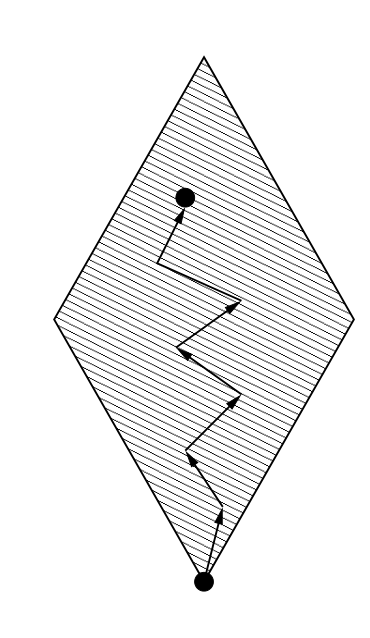
\includegraphics[width=0.2\textwidth]{figures/fixed-point_walk}
\end{center}
\caption{A walk through the lattice, starting a $\bot$ and ending in the fixed-point}
\label{lattice_walk}
\end{figure}
